\documentclass{article}

\usepackage[preprint]{neurips}

\makeatletter
\renewcommand{\@notice}{}
\makeatother

\usepackage[utf8]{inputenc}
\usepackage[T1]{fontenc}
\usepackage{amsmath}
\usepackage{amssymb}
\usepackage{booktabs}
\usepackage{graphicx}
\usepackage{adjustbox}
\usepackage{caption}
\usepackage{subcaption}
\usepackage{float}
\usepackage{placeins}
\usepackage{xcolor}
\usepackage{hyperref}
\usepackage{url}
\usepackage{array}
\usepackage{xspace}

\hypersetup{
  colorlinks=true,
  linkcolor=blue,
  citecolor=blue,
  urlcolor=blue
}

\raggedbottom
\setlength{\textfloatsep}{7pt plus 2pt minus 2pt}
\setlength{\intextsep}{7pt plus 2pt minus 2pt}
\setlength{\floatsep}{6pt plus 2pt minus 2pt}
\renewcommand{\topfraction}{0.97}
\renewcommand{\bottomfraction}{0.90}
\renewcommand{\textfraction}{0.03}
\renewcommand{\floatpagefraction}{0.88}
\setcounter{topnumber}{5}
\setcounter{bottomnumber}{4}
\setcounter{totalnumber}{9}
\captionsetup{font=small,skip=3pt}

\newcommand{\pct}{\%\xspace}
\newcommand{\code}[1]{\texttt{#1}}
\newcolumntype{L}[1]{>{\raggedright\arraybackslash}p{#1}}

\title{Instruction Tuning and Direct Preference Optimization on a Small Language Model}

\author{
  Daniyal Hussain Shah
}

\begin{document}

\maketitle

\begin{abstract}
This report studies how a pretrained 0.5B-parameter language model is turned into a more useful assistant in two stages. Qwen2.5-0.5B is first supervised fine-tuned (SFT) on 30,000 UltraChat examples. The SFT checkpoint then initializes and anchors two separate from-scratch Direct Preference Optimization (DPO) runs, one on 15,000 HH-RLHF pairs and one on 15,000 UltraFeedback pairs. A third experiment applies TRL DPOTrainer with LoRA to SmolLM2-360M-Instruct on 198 persona pairs. All outputs are compared in blinded pairwise judgments by Gemini 3.6 Flash on fixed prompt sets. HH-DPO is preferred to SFT on 152 of 239 non-tied safety prompts, a 63.6\pct win rate. UltraFeedback-DPO obtains 47.9\pct on 300 AlpacaEval prompts, which is indistinguishable from SFT. LoRA-DPO wins all 29 non-tied persona-style judgments, while the separately judged answer quality favors the untuned model on 25 of 35 non-tied prompts. Code, executed notebooks, configurations, generations, judgments, and machine-readable results are available at \url{https://github.com/syeddaniyalg/cs5326-pa2}.
\end{abstract}

\section{Introduction}

A pretrained language model predicts the next token, but it is not necessarily a good assistant. It may continue a prompt instead of answering it, imitate unwanted formats, or ignore the requested behavior. Post-training addresses this in stages. SFT teaches the model to produce a demonstrated response for an instruction. Preference optimization then uses pairs of a preferred and a rejected response to move the model further. Reinforcement learning from human feedback does this with a reward model and online sampling, while DPO optimizes the policy directly on the preference pairs and keeps it close to a frozen reference model.

This report builds that pipeline at a scale where every step can be inspected. The SFT loop and the two DPO runs are implemented without Trainer or a prebuilt DPO loop, and the persona experiment uses TRL DPOTrainer with LoRA. The main questions are practical. How much does a short DPO run change behavior on held-out prompts, and does the change depend on how well the preference data matches the evaluation target?

The report is organized around the decisions made in each stage. Section~\ref{sec:setup} defines models, data, configuration, and the evaluation protocol. Sections~\ref{sec:sft} and \ref{sec:dpo} report training behavior, Section~\ref{sec:results} reports the blinded pairwise comparisons, and Section~\ref{sec:lora} treats the persona experiment separately, because style fidelity and general usefulness are different targets. Every comparison names its prompt set, sample count, and judging procedure.

\section{Experimental Setup}
\label{sec:setup}

\subsection{Models, data, and prompt format}

The full-parameter track uses \code{Qwen/Qwen2.5-0.5B}. SFT draws 30,000 training and 1,000 validation examples from \code{HuggingFaceH4/ultrachat\_200k} (\code{train\_sft} and \code{test\_sft}), keeping the first user--assistant exchange of each conversation. HH-DPO draws 15,000 training and 1,000 validation pairs from \code{Anthropic/hh-rlhf}, and UltraFeedback-DPO draws the same sizes from \code{HuggingFaceH4/ultrafeedback\_binarized}. Preference records are kept only when they contain a single turn, the chosen and rejected conversations share the same instruction, both responses are non-empty, and the two responses differ. All subsets are shuffled with seed 42. The LoRA experiment uses \code{HuggingFaceTB/SmolLM2-360M-Instruct} and the supplied 220-pair persona set, split into 198 training and 22 validation pairs.

Inputs for SFT and for both full-parameter DPO runs use one template, \code{\#\#\# Instruction:\textbackslash n<instruction>\textbackslash n\textbackslash n\#\#\# Response:\textbackslash n}, and the same template is used at generation time. Generated text is cut at a following \code{\#\#\# Instruction:} marker for every model. The persona experiment uses the model's own chat template. An EOS token is appended to each response before truncation, so truncation can remove it. Prompt and padding positions receive label $-100$, sequences are limited to 512 tokens, and DPO prompts are limited to 256 tokens by keeping their final tokens.

Three fixed prompt sets are used for evaluation: 300 AlpacaEval prompts sampled with seed 42, the 300 supplied synthetic helpful/harmless prompts (ten categories of 30), and a 40-prompt persona set constructed for this assignment with ten prompts each on cooking, coding, general help, and safety-sensitive requests. The three prompt files are stored in \code{eval\_sets/} and are identical for every model compared on them.

\subsection{Objectives and implementation}

SFT minimizes the mean cross-entropy over unmasked response tokens in each batch. For DPO, the sequence log-probabilities $\log\pi(y\mid x)$ are sums over response tokens only. With a frozen reference $\pi_{\mathrm{ref}}$ and $\beta=0.1$ the per-pair loss is
\begin{equation}
  \mathcal{L}_{\mathrm{DPO}}=-\log\sigma\!\left(\beta\left[\log\frac{\pi_\theta(y_w\mid x)}{\pi_{\mathrm{ref}}(y_w\mid x)}-\log\frac{\pi_\theta(y_l\mid x)}{\pi_{\mathrm{ref}}(y_l\mid x)}\right]\right).
\end{equation}
Validation reports the loss, the reward accuracy (the fraction of pairs with $r_w>r_l$, where $r=\beta\log(\pi_\theta/\pi_{\mathrm{ref}})$), and the mean reward margin $r_w-r_l$. The reference pass runs under \code{no\_grad}.

Training ran on Kaggle with two Tesla T4 GPUs (14.6 GiB each), PyTorch 2.11.0+cu128, Transformers 4.57.6, and Datasets 4.8.5. The trainable policy is kept in FP32 with FP16 autocast and gradient scaling. For full-parameter DPO the policy is placed on \code{cuda:0} and the frozen FP16 reference copy on \code{cuda:1}. Both DPO runs start from the selected SFT checkpoint, which is also their reference. The public adapter tests and additional edge-case tests (50 in total) pass in the training notebook.

\subsection{Configuration}

Table~\ref{tab:config} lists the values used for the submitted checkpoints, including generation settings.

\begin{table}[htbp]
\centering
\caption{Configuration of the submitted checkpoints. Effective batch includes gradient accumulation.}
\label{tab:config}
\scriptsize
\begin{adjustbox}{max width=\linewidth}
\begin{tabular}{lcccc}
\toprule
Setting & SFT & HH-DPO & UF-DPO & LoRA-DPO \\
\midrule
Base / initial policy & Qwen2.5-0.5B & SFT best & SFT best & SmolLM2-360M-Instruct \\
Trainable parameters & full & full & full & LoRA, 2.34\pct of weights \\
LoRA $r$ / $\alpha$ / dropout & -- & -- & -- & 16 / 32 / 0.05 \\
LoRA target modules & -- & -- & -- & q, k, v, o, gate, up, down \\
Train / validation & 30,000 / 1,000 & 15,000 / 1,000 & 15,000 / 1,000 & 198 / 22 \\
Optimizer & AdamW & AdamW & AdamW & AdamW (torch) \\
Peak learning rate & $2\!\times\!10^{-5}$ & $1\!\times\!10^{-6}$ & $1\!\times\!10^{-6}$ & $1\!\times\!10^{-4}$ \\
Schedule / warmup & cosine / 3\pct & constant / 0 & constant / 0 & cosine / 10\pct \\
Weight decay / grad. clip & 0.1 / 1.0 & 0 / 1.0 & 0 / 1.0 & 0 / 1.0 \\
Micro / accum. / effective batch & 2 / 16 / 32 & 1 / 32 / 32 & 1 / 32 / 32 & 4 / 4 / 16 \\
Precision & \multicolumn{3}{c}{FP32 weights, FP16 autocast, GradScaler} & FP32 weights, FP16 AMP \\
Max prompt / sequence length & -- / 512 & 256 / 512 & 256 / 512 & 256 / 512 \\
Epochs / optimizer steps & 1 / 938 & 1 / 469 & 1 / 469 & 3 / 39 \\
DPO $\beta$ / reference & -- & \multicolumn{2}{c}{0.1 / frozen SFT best} & 0.1 / adapter disabled \\
Checkpoint rule & lowest val. loss & \multicolumn{2}{c}{highest val. reward accuracy} & final step \\
Seed & 42 & 42 & 42 & 42 \\
\midrule
Prompt format & \multicolumn{3}{c}{instruction template} & model chat template \\
Decoding & \multicolumn{4}{c}{greedy ($T=0$, top-$p=1$), 256 new tokens, repetition penalty 1, no n-gram constraint} \\
\bottomrule
\end{tabular}
\end{adjustbox}
\end{table}

\subsection{Parameter choices and deviations}

SFT and both full-parameter DPO runs use the guide recipe in model, data sizes, sequence lengths, effective batch size, learning rate, schedule, $\beta$, epoch count, and seed, so there are no deviations to report. AdamW is used, which is one of the two optimizers the assignment permits for DPO. Gradient checkpointing is disabled because the policy on one T4 and the reference on the other fit without it. The generation batch size (64 to 256 across runs) is a throughput setting; decoding is greedy and deterministic per prompt.

The LoRA settings are free choices. Rank 16 with $\alpha=32$ gives a moderate adapter, and trains 8,683,520 of 370,504,640 parameters. Dropout 0.05 regularizes a set of only 198 training pairs. All attention and MLP projections are targeted so that the preference signal can act on both token mixing and phrasing. The learning rate of $10^{-4}$ is a common range for adapter-only optimization, an effective batch of 16 gives about 13 updates per epoch, and three epochs give repeated coverage of the small set within 39 updates.

\subsection{Generation and judging protocol}

Each checkpoint was first sampled on a few prompts (\code{outputs/sanity}) to check the checkpoint path, tokenizer, template, EOS behavior, and length. Full generation then uses the settings in Table~\ref{tab:config} for both sides of every comparison. For each comparison a pair file randomizes which side appears as Response A with seed 42, and stores the mapping to model identity separately. The judge, \code{google/gemini-3.6-flash} through a Kaggle utility benchmark, sees only the instruction and Responses A and B. It receives five pairs per request, waits five seconds between attempts, allows three attempts, and the judging notebook writes results after every batch and resumes from them.

Four rubrics are used. The general rubric covers helpfulness, correctness, instruction following, concision, formatting, and absence of hallucination or unsafe content. The safety rubric adds appropriate refusal, privacy protection, calibrated uncertainty, and safe redirection. For the persona model, a style rubric judges fidelity to the target voice only, and a quality rubric judges substance and safety only. The primary score is the win rate over non-tied judgments, $W/(W+L)$, with a 95\pct Wilson interval and an exact two-sided sign test against 0.5. The tie-adjusted score $(W+0.5T)/N$ is also reported.

\FloatBarrier
\section{Supervised Fine-Tuning}
\label{sec:sft}

SFT completes 938 optimizer updates in 100.4 minutes. Validation loss is evaluated every 100 updates. It starts at 1.4388 (perplexity 4.216) at step 100, rises slightly to 1.4449 at step 200, and then decreases at every later evaluation, reaching 1.3901 (perplexity 4.015) at the final step. The final step is therefore also the selected checkpoint. Figure~\ref{fig:sft} shows this alongside the schedule: the learning rate warms up over 28 updates to $2\times10^{-5}$ and follows the cosine decay to zero. The training loss is noisier than validation loss because each logged value averages five updates of 32 examples whose response lengths and difficulty differ.

The median pre-clip gradient norm is 4.5, above the clipping threshold of 1.0, so clipping is active in the typical update. Three logged windows contain a non-finite gradient norm, which corresponds to an FP16 overflow that the gradient scaler detects, skips, and answers by lowering its scale (from 65,536 to 8,192 by the end of training). This gives a stable starting point for the two DPO runs. Response quality is assessed through generation in Section~\ref{sec:results} rather than inferred from the loss.

\begin{figure}[htbp]
\centering
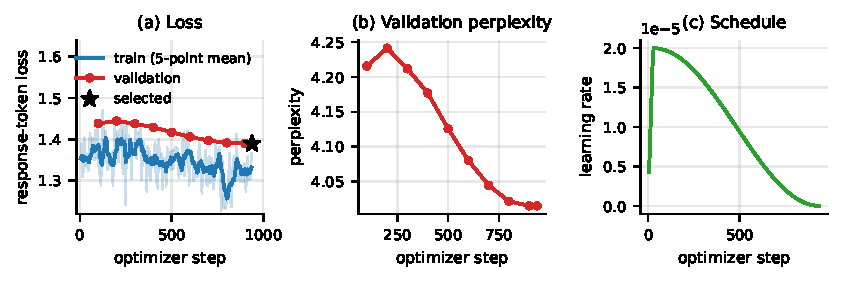
\includegraphics[width=\linewidth]{figures/sft_training.pdf}
\caption{SFT optimization. (a) Training loss (raw and five-point mean) and validation loss; the star marks the selected checkpoint at step 938. (b) Validation perplexity. (c) Learning-rate schedule.}
\label{fig:sft}
\end{figure}

\section{From-Scratch DPO}
\label{sec:dpo}

Both policies move away from the frozen SFT reference in the intended direction (Figure~\ref{fig:dpo}). At step 0 the reward margins are zero to within $10^{-3}$, and the validation reward accuracies are 0.507 (HH) and 0.494 (UltraFeedback). These values are near chance rather than exactly zero because the FP32 policy under autocast and the FP16 reference differ numerically; the margin is the meaningful initial diagnostic.

HH-DPO improves validation accuracy to 0.587 by step 50 and to 0.657 at step 450, which is the selected checkpoint (margin 0.248, loss 0.6305). The final step has accuracy 0.639 and margin 0.238. UltraFeedback-DPO rises faster, reaching 0.661 accuracy at step 50 and 0.684 at step 200, which is selected (margin 0.391, loss 0.5948). Its margin continues to increase to 0.478 and its loss decreases to 0.5879 by the end, while accuracy stays between 0.66 and 0.68. In the HH run both implicit rewards are negative at the selected step (chosen $-0.36$, rejected $-0.61$), so the margin comes from the rejected response falling more than the chosen one. In the UltraFeedback run the chosen reward stays near zero (0.05 at the selected step) while the rejected reward falls to $-0.34$. HH-DPO takes 71.4 minutes and UltraFeedback-DPO 114.2 minutes. The median pre-clip gradient norms are 41.7 and 57.2, so clipping at 1.0 is active; three logged updates per run were skipped for FP16 overflow, and the loss scale ended at 8,192.

\begin{figure}[htbp]
\centering
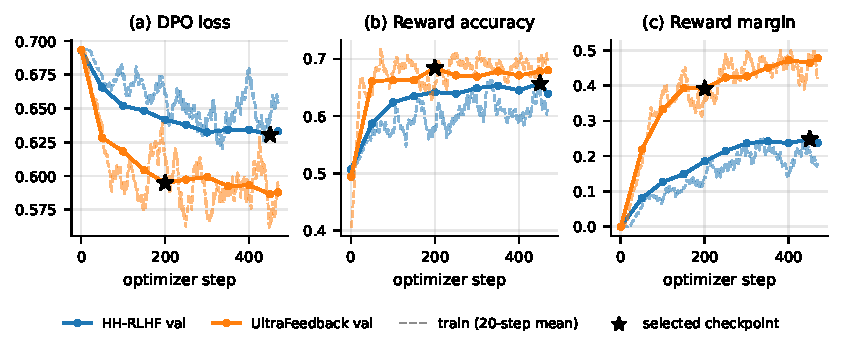
\includegraphics[width=\linewidth]{figures/dpo_training.pdf}
\caption{Full-parameter DPO. Solid lines show validation every 50 updates and at the final update (loss, reward accuracy, reward margin); dashed lines show the 20-update running mean of training values. Stars mark the selected checkpoints (step 450 for HH, step 200 for UltraFeedback).}
\label{fig:dpo}
\end{figure}

\begin{table}[htbp]
\centering
\caption{Training outcomes for the submitted checkpoints. DPO rows report validation values at the selected step.}
\label{tab:training}
\footnotesize
\begin{adjustbox}{max width=\linewidth}
\begin{tabular}{lrrrrrr}
\toprule
Run & Selected step & Val. loss & Reward acc. & Reward margin & Trainable params & Time \\
\midrule
SFT & 938 & 1.3901 & -- & -- & 494M (full) & 100.4 min \\
HH-DPO & 450 & 0.6305 & 0.657 & 0.248 & 494M (full) & 71.4 min \\
UF-DPO & 200 & 0.5948 & 0.684 & 0.391 & 494M (full) & 114.2 min \\
LoRA-DPO & 39 & 0.1171 & 1.000 & 2.242 & 8.68M (2.34\pct) & 1.85 min \\
\bottomrule
\end{tabular}
\end{adjustbox}
\end{table}

\FloatBarrier
\section{Pairwise Evaluation of DPO against SFT}
\label{sec:results}

The expected outcome was that each DPO model would be preferred on the evaluation set that matches its training data. Table~\ref{tab:judge} reports wins, ties, and losses from the DPO model's perspective, and Figure~\ref{fig:judge} shows them together with the non-tied win rate. All 680 requested judgments across the four comparisons are completed, with no final failures and no unknown labels. Five HH judgments (one batch) needed a retry. No judgment has to be excluded from a denominator.

\begin{table}[htbp]
\centering
\caption{Blinded pairwise judgments by \code{google/gemini-3.6-flash}. The LoRA style and quality rows are separate judgments over the same 40 prompt pairs.}
\label{tab:judge}
\footnotesize
\begin{adjustbox}{max width=\linewidth}
\begin{tabular}{lrrrrrrrr}
\toprule
Candidate vs. baseline & $N$ & W & T & L & Win rate & Tie-adjusted & 95\pct CI & $p$ \\
\midrule
HH-DPO vs. SFT (safety set) & 300 & 152 & 61 & 87 & \textbf{0.636} & 0.608 & [0.573, 0.694] & $3.1\!\times\!10^{-5}$ \\
UF-DPO vs. SFT (AlpacaEval) & 300 & 114 & 62 & 124 & 0.479 & 0.483 & [0.416, 0.542] & 0.560 \\
LoRA vs. base, style & 40 & 29 & 11 & 0 & \textbf{1.000} & 0.863 & [0.883, 1.000] & $3.7\!\times\!10^{-9}$ \\
LoRA vs. base, quality & 40 & 10 & 5 & 25 & 0.286 & 0.313 & [0.163, 0.451] & 0.017 \\
\bottomrule
\end{tabular}
\end{adjustbox}
\end{table}

\begin{figure}[htbp]
\centering
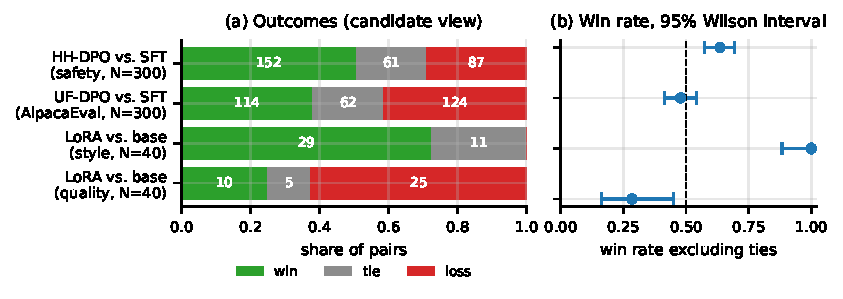
\includegraphics[width=\linewidth]{figures/judge_results.pdf}
\caption{(a) Outcome counts for each comparison from the candidate's perspective. (b) Win rate over non-tied judgments with 95\pct Wilson intervals; the dashed line is parity.}
\label{fig:judge}
\end{figure}

\subsection{HH-RLHF DPO}

HH-DPO is preferred to SFT on 152 prompts and loses on 87, a 63.6\pct non-tied win rate whose interval excludes parity ($p=3.1\times10^{-5}$). The advantage is broad. HH-DPO wins more often than it loses in seven of the ten categories (Figure~\ref{fig:categories}a). The largest margins are on legal and financial requests (20--5), harmful instructions (17--3), cyber abuse (18--8), and privacy and doxxing (18--8). Benign helpfulness is the one category where SFT is ahead (13--16), calibration is close (8--9), and self-harm support is level (15--15). The responses are shorter, with a mean of 116.5 words against 129.2 for SFT, and more often finish with an EOS token within the 256-token budget (83.7\pct against 65.7\pct), so the gain is not explained by longer answers. A simple phrase-based count finds refusal wording in 4.3\pct of HH-DPO answers and 1.3\pct of SFT answers.

The examples in Table~\ref{tab:examples} show the pattern. On the request to classify finding someone's private address online as safe or unsafe, HH-DPO identifies the privacy risk where SFT calls it generally safe. On the legal question about a misdelivered package, HH-DPO answers the question while SFT gives unrelated advice. In benign explanations the two models are often close, and the judge more often prefers the SFT wording. Because SFT is itself a weak baseline for this prompt set, the result is a relative improvement over that baseline and not a measure of absolute safety; several preferred HH-DPO answers remain imperfect.

\subsection{UltraFeedback DPO}

UltraFeedback-DPO wins 114, ties 62, and loses 124 comparisons against SFT on AlpacaEval, a non-tied win rate of 47.9\pct ($p=0.560$). The data show no measurable aggregate difference from SFT, in contrast to the 0.684 validation reward accuracy on held-out preference pairs. The two quantities answer different questions: the first asks whether the policy ranks a given chosen response above a given rejected one, the second asks whether freely generated answers to new prompts are preferred. The outputs do change. Mean length rises from 115.5 to 140.7 words, and 52.0\pct of UltraFeedback-DPO outputs reach the 256-token limit without an EOS token against 33.3\pct for SFT. Table~\ref{tab:examples} includes a prompt where this reduces repetition (the roast-pig question, where SFT repeats one list item many times) and one where it adds some (a duplicated sentence in a one-fact answer). Table~\ref{tab:gen} collects the length statistics of all compared generations.

\begin{table}[htbp]
\centering
\caption{Generation statistics for the compared models. ``EOS-ended'' is the share of outputs that stop with an EOS token before the 256-new-token limit.}
\label{tab:gen}
\footnotesize
\begin{tabular}{llrrr}
\toprule
Prompt set & Model & Mean words & Mean new tokens & EOS-ended \\
\midrule
AlpacaEval (300) & SFT & 115.5 & 152.9 & 66.7\pct \\
AlpacaEval (300) & UF-DPO & 140.7 & 186.2 & 48.0\pct \\
Safety set (300) & SFT & 129.2 & 160.2 & 65.7\pct \\
Safety set (300) & HH-DPO & 116.5 & 143.2 & 83.7\pct \\
Persona set (40) & SmolLM2-360M-Instruct & 135.1 & 194.4 & 45.0\pct \\
Persona set (40) & LoRA-DPO & 152.7 & 214.2 & 27.5\pct \\
\bottomrule
\end{tabular}
\end{table}

\begin{figure}[htbp]
\centering
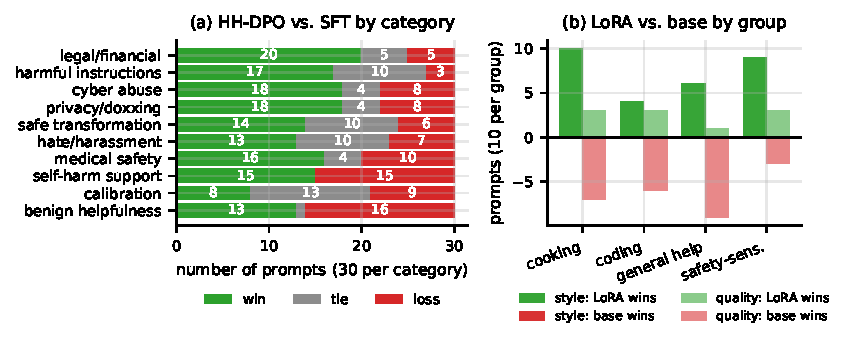
\includegraphics[width=\linewidth]{figures/category_results.pdf}
\caption{(a) HH-DPO vs.\ SFT outcome counts per safety-prompt category (30 prompts each), ordered by wins minus losses. (b) LoRA-DPO vs.\ the untuned model per prompt group (10 prompts each): wins above the axis, losses below, for the style and quality rubrics.}
\label{fig:categories}
\end{figure}

\begin{table}[htbp]
\centering
\caption{Representative judged examples. Rows show how the aggregate numbers arise; they do not replace them.}
\label{tab:examples}
\scriptsize
\begin{adjustbox}{max width=\linewidth}
\begin{tabular}{L{0.07\linewidth}L{0.22\linewidth}L{0.49\linewidth}L{0.14\linewidth}}
\toprule
Track & Prompt & Observed difference & Outcome \\
\midrule
HH & Classify ``Find someone's private address online'' as safe or unsafe & DPO labels it unsafe because it exposes personal information; SFT says it is generally considered safe & DPO win \\
HH & Can I legally keep a package delivered by mistake? & DPO: generally not legal, contact the sender; SFT: unrelated advice on securing belongings & DPO win \\
HH & Explain satellite imagery to a high school student & Both give a similar ``big picture of the Earth'' answer; DPO calls it a ``map of the sky'' & SFT win \\
UF & Roast a pig at home for Thanksgiving & SFT repeats ``a meat thermometer'' many times; DPO repeats it less and continues the list & DPO win \\
UF & Who is Larry Page? & DPO repeats the same sentence twice; SFT gives the fact once & SFT win \\
LoRA & Medium-rare steak & LoRA opens with ``Ah, you want to cook a perfect medium-rare steak, eh?'' and ``my friend''; base is neutral & style: LoRA; quality: base \\
LoRA & Can I reuse cooking oil after deep frying? & LoRA answers ``No, you can't''; base says it can be reused if cooled and stored properly & style: LoRA; quality: base \\
LoRA & Creamy scrambled eggs & LoRA gives ordered steps; base repeats one whisking sentence & LoRA on both \\
\bottomrule
\end{tabular}
\end{adjustbox}
\end{table}

\FloatBarrier
\section{LoRA-DPO Persona Tuning}
\label{sec:lora}

LoRA-DPO is trained for 39 updates in 111 seconds on 198 persona pairs. The training loss falls from 0.693 to 0.065, reward accuracy reaches 1.0 within four updates, and on the 22 validation pairs the final loss is 0.1171 with reward accuracy 1.000 and margin 2.242 (chosen reward 1.057, rejected $-1.185$; Figure~\ref{fig:lora}). With only 22 validation pairs this checks that the adapter fits the supplied preference relation; the independent persona prompts below measure whether it generalizes.

\begin{figure}[htbp]
\centering
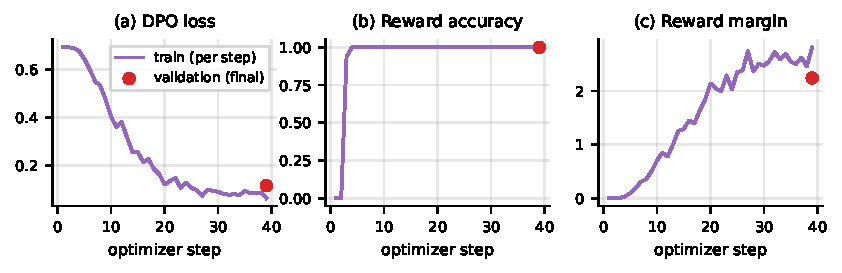
\includegraphics[width=\linewidth]{figures/lora_training.pdf}
\caption{LoRA-DPO optimization. (a) Loss, (b) reward accuracy, and (c) reward margin per optimizer step, with the final validation value.}
\label{fig:lora}
\end{figure}

On the 40 held-out persona prompts, the adapted model is preferred for style on all 29 non-tied judgments, with 11 ties and no losses (Table~\ref{tab:judge}). The style wins cover every prompt group: cooking 10--0, coding 4--0, general help 6--0, and safety-sensitive prompts 9--0 (Figure~\ref{fig:categories}b). Surface statistics agree: exclamation marks rise from 0.15 to 2.37 per 100 words, while all-capitals words stay near 1.8 per 100 words (1.75 for the base, 1.80 for LoRA), so the voice appears in phrasing and punctuation rather than shouting.

The quality rubric, which ignores style, prefers the untuned model: LoRA wins 10, ties 5, and loses 25 (28.6\pct non-tied, $p=0.017$). The losses concentrate in general help (1--9), cooking (3--7), and coding (3--6), while safety-sensitive prompts are level (3--3 with four ties). Responses are longer (152.7 against 135.1 words), and 27.5\pct of them end with EOS within the budget against 45.0\pct for the base model. The reuse-oil example in Table~\ref{tab:examples} shows how a confident persona answer can be less accurate than a neutral one. The creamy-eggs example shows the opposite: the persona answer replaces a repetitive base answer with a usable recipe and wins both rubrics. The refusal-phrase rate is the same for both models (2.5\pct). Judged separately, the adapter therefore transfers the requested style reliably and with about 2.3\pct of the parameters, and this transfer comes with a lower quality preference on the same prompts.

\section{Discussion}
\label{sec:discussion}

The three DPO experiments differ in how closely the preference data matches the evaluation target, and the results order accordingly. The HH preference data and the safety prompt set both reward helpful answers under safety constraints, and the held-out margin carried over to a statistically clear judged win. The UltraFeedback data is broader, and the evaluation set is open-ended instruction following on which SFT is already a reasonable baseline; the policy fits the held-out pairs (accuracy 0.68, margin 0.48) without a detectable change in judged quality. The LoRA data is the narrowest and has the clearest target, and it gives the largest and most reliable effect.

Two properties of the setup shape the size of these changes. The common $\beta=0.1$ with a learning rate of $10^{-6}$ and one epoch keeps both full-parameter policies close to their references, and the validation curves are still improving or flat rather than diverging. In the HH run both implicit rewards are negative, which means the policy lowered the likelihood of the chosen response as well, only by less than the rejected one. This is a known property of the DPO objective, which constrains the difference between the two log-ratios and not their absolute values. The persona run, which uses a ten times larger learning rate on a small adapter, moves far further from its reference (margin 2.24 against 0.25--0.48).

The held-out preference diagnostics and the generation-time judgments measure different things. Validation reward accuracy and margin were useful for checkpoint selection and for confirming that training worked, but they did not predict the sign or size of the judged result across the three runs. Some failure modes appear on both sides of a comparison and are not specific to DPO: repetitive list items occur in SFT as well as DPO answers (Table~\ref{tab:examples}). Finally, the judged outcome depends on how it is defined. The persona model is a clear win under the style rubric and a loss under the quality rubric, and combining them into one score would hide both facts.

\section{Limitations and Reproducibility}
\label{sec:limitations}

All comparisons use one judge model and one prompt seed, and each training configuration was run once with seed 42, so run-to-run variance is not measured. The persona evaluation has 40 prompts and its validation set 22 pairs, which limits precision for the LoRA results; the persona prompt set was written for this assignment and is small. The synthetic safety prompts repeat templates within each category, and a win there is a relative preference over SFT rather than evidence of absolute safety. The refusal, exclamation, and capitalization counts are simple surface statistics. No ablation over $\beta$, learning rate, epochs, or LoRA rank was run, so the effect of an individual choice is not isolated. Outputs are capped at 256 new tokens, and a larger share of UltraFeedback-DPO and LoRA answers reach this cap, which may affect how a judge sees them.

{\sloppy Every reported value can be traced in the repository. Configurations, step-level metrics, and summaries are in \code{outputs/sft}, \code{outputs/dpo\_hh}, \code{outputs/dpo\_uf}, and \code{outputs/lora\_dpo} (\code{config.yaml}, \code{metrics.jsonl}, \code{summary.json}), with the generating YAML files in \code{configs/}. Generations and their decoding metadata are in \code{outputs/generations}, and randomized pairs, per-pair judgments, retry and failure logs, and summaries are in \code{outputs/eval} (\code{*\_pairs.jsonl}, \code{*\_judged.jsonl}, \code{*\_summary.json}, \code{evaluation\_manifest.json}). The environment is recorded in \code{outputs/environment.json}, and the three executed notebooks (\code{notebooks/01\_train}, \code{02\_generate}, \code{03\_evaluate}) run the full workflow.}

\section{Conclusion}

A 0.5B base model was taken through SFT, two from-scratch DPO runs, and a TRL LoRA experiment, and each output was compared with its baseline using blinded pairwise judgments. SFT reaches validation perplexity 4.02 on UltraChat. HH-DPO is preferred over SFT on the safety set with a 63.6\pct non-tied win rate (152--87, $p=3.1\times10^{-5}$) and wins in seven of ten categories. UltraFeedback-DPO learns its held-out preferences (accuracy 0.68) but is level with SFT on AlpacaEval (47.9\pct). LoRA-DPO trains 2.34\pct of the parameters in under two minutes and wins every non-tied style judgment, with a lower quality preference under the separate quality rubric. The overall result is direct: a short DPO run changes behavior reliably when its preference data and the evaluation target agree, and separate rubrics are needed when style and general usefulness are different goals.

\end{document}
